%!TEX root = ../paper.tex

\centering
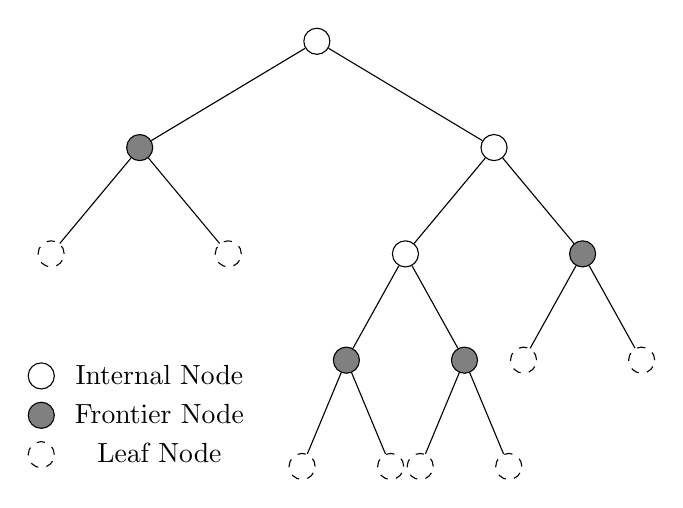
\begin{tikzpicture}[scale=.9,level/.style={sibling distance=50mm/#1}]
\node [circle,draw] (z) {}
  child {node [circle,draw,fill=gray] (a) {}
    child {node [circle,draw,dashed] (b) {}}
    child {node [circle,draw,dashed] (g) {}}
  }
  child {node [circle,draw] (j) {}
    child {node [circle,draw] (k) {}
      child {node [circle,draw,fill=gray] (o) {}
        child {node [circle,draw,dashed] (x) {}}
        child {node [circle,draw,dashed] (y) {}}
      }
      child {node [circle,draw,fill=gray] (p) {}
        child {node [circle,draw,dashed] (x) {}}
        child {node [circle,draw,dashed] (y) {}}
      }
    }
  child {node [circle,draw,fill=gray] (l) {}
    child {node [circle,draw,dashed] (c) {}}
    child {node [circle,draw,dashed] (d) {}}
  }
};

\node [shift={(-3.5,-4.25)},circle,draw,label={[xshift=1.5cm, yshift=-0.4cm] Internal Node}] (leg1) {};
\node [shift={(-3.5,-4.75)},circle,draw,fill=gray,label={[xshift=1.5cm, yshift=-0.4cm] Frontier Node}] (leg1) {};
\node [shift={(-3.5,-5.25)},circle,draw,dashed,label={[xshift=1.5cm, yshift=-0.4cm] Leaf Node}] (leg1) {};
\end{tikzpicture}
